\documentclass[a4paper, oneside]{memoir}
\usepackage[top=25mm, bottom=25mm]{geometry}	% layout margin
\usepackage{graphicx}
\graphicspath{ {./images/} }

\title{How to write a Report\\ for the Project of Distributed Systems}

\author{Prof. Marino Miculan\\ DMIF, University of Udine, Italy}

\date{Version 0.2, \today}

\begin{document}


%\begin{titlingpage}
\maketitle
%\begin{abstract}
%\end{abstract}
%\end{titlingpage}

\chapter{Introduction}\label{ch:intro}

%In this chapter you describe the main problem, and an idea of the solution. It is not necessary to be very detailed or formal, but it is important to explain which are the main aims and issues from the point of view of Distributed Systems:
%\begin{itemize}
%A description of the application.
%The overall structure of the implementation: how resources are deployed, which are the players, the roles.
%\item The distributed system features (and the transparencies) and algorithms you intend to implement.
%\item Your plan for testing the system.
%\item A schedule for how you plan to carry our your design and implementation
%\end{itemize}

\section{Description of the application.}
The problem to solve is the delivery of packages and management of a dynamic fleet of drones.

The space is modelled by a 2D grid, so the diagonal movements of drones are calculated with some approximation. There aren't forbidden zones nor forced paths.

The drones have cellular connectivity and know a few other drones. They are equipped with GPS and we assume they have an ID, it's not a limitation since the ID could be given by the manager server (see below).

There are some recharging and repairing stations on the map. For simplicity the recharging stations and warehouses are assumed to have unlimited capacity.

There is a server that centralize the orders of the clients and act as a reliable message broker (as middle-man).

There is a server which provide some management of drones, and make sure the order is carried out. In particular, the tracker functionality, when a new drone is connected the server will provide a list of other drones to connect to and the locations of recharging/repairing stations.

\begin{figure}[h!]
	\centering
	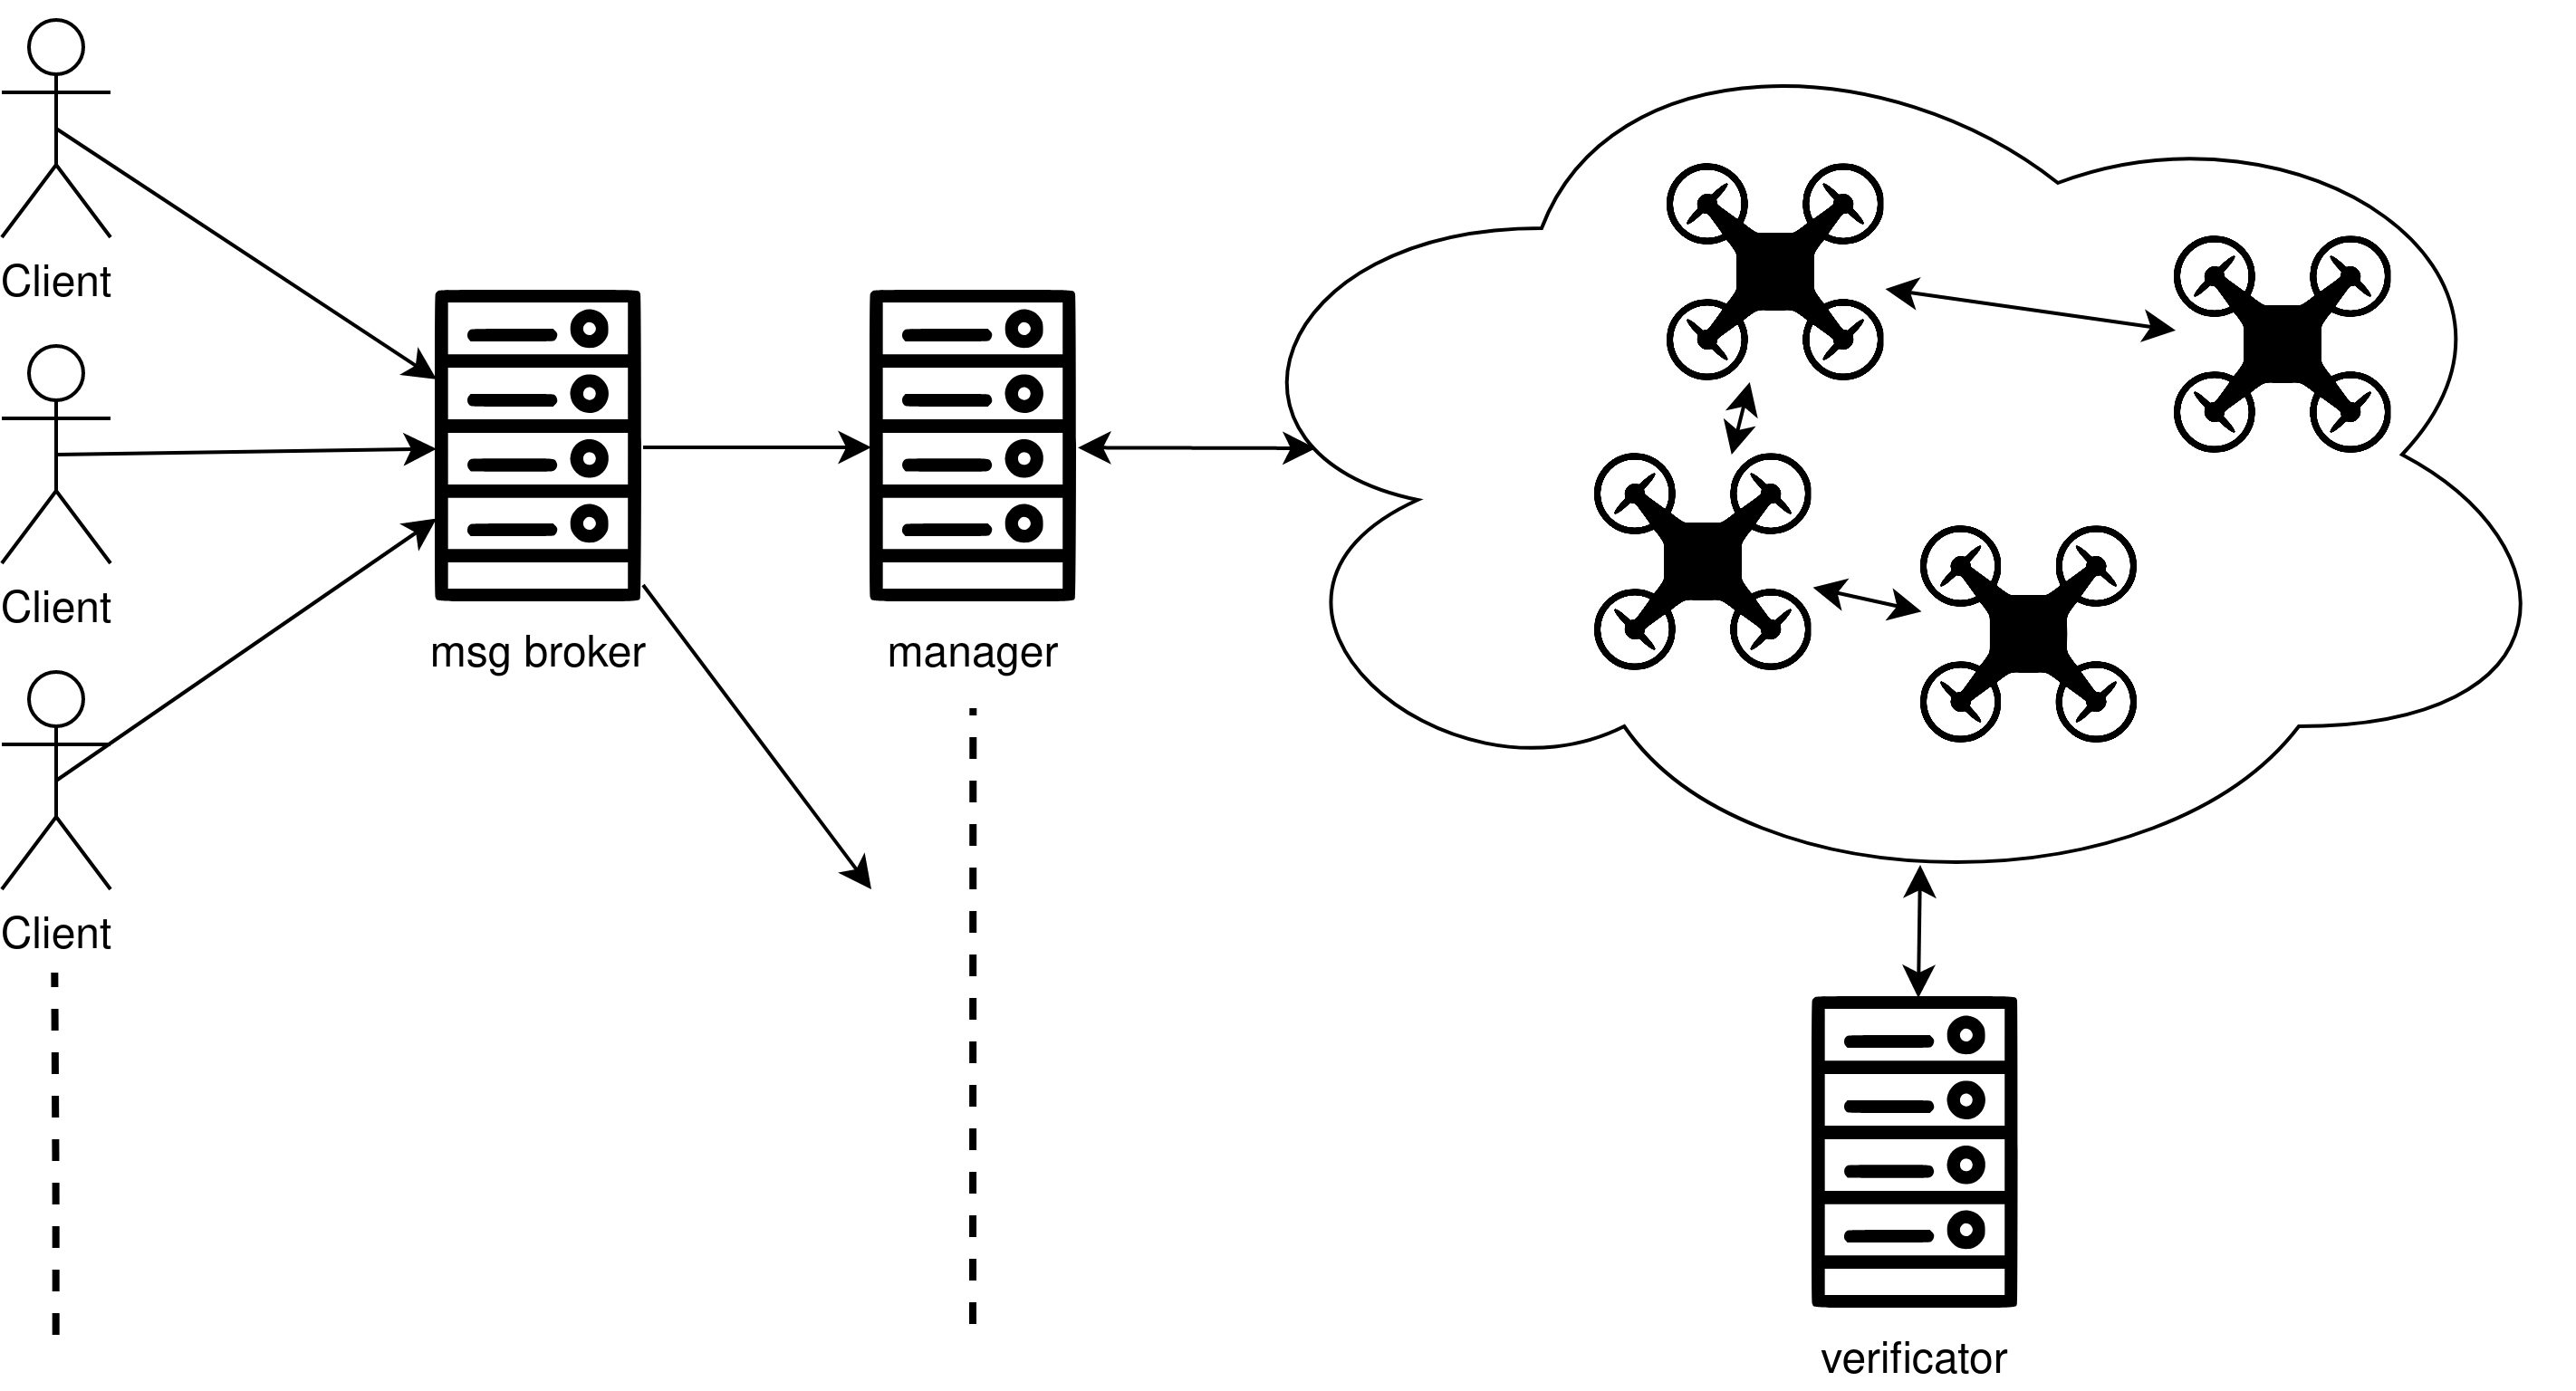
\includegraphics[width=\linewidth]{Overview}
\end{figure}

A client can send a request to the broker server for the delivery of a package from point A to point B, a drone will be selected based on its position relative to point A, its  battery and maximum carry weight, the selected drone will carry out the delivery of the package.

If a drone has low battery it will enter reserve mode, it will locate the nearest charging station and it will move in that direction, the charging stations are fixed and their location is known to all drones.

A drone can crash at any point in time, if it was able to signal the fail, another drone will be selected to transport the broken drone to the nearest charging station, if the broken drone was satisfying a request a second drone will be selected to complete the task.


\section{Structure of the implementation}

The client position is not considered in our system, drones can be in any point in the map and move only if they need to deliver a package or if they need to recharge, the charging stations are located in fixed points in the map, their position is known to all drones.

The key players in our implementation are:
\begin{itemize}
\item "Client": the client sends a request to the broker server for a delivery. It's also able to query the broker asking for the status of the delivery;
\item "Drone": the drones are the entities that move the packages between locations, new drones that want to join the network send a message to the manager server, drones with low battery must go to a charging station to recharge;
\item "Broker server": this server receives the requests from clients, it's a single point of failure so it is replicated by a backup copy (it's possible to have more copies);
\item "Manager server": this server handles the entry of a new drone in the network, a drone can have it's own unique id or can obtain one from this server. Other functionalities are the detection of an offline drone and consequentially offers the best-effort guarantee of successful delivery. The server is a single point of failure so it is replicated by a backup copy (it's possible to have more copies);
\item "Recharging/Repairing station": these are stations in fixed points in the map where drones can go to recharge their battery and where broken drones can be brought for repairs.
\end{itemize}


\section{System features and algorithms}


The system transparencies that we aim to implement are:
\begin{itemize}
	\item concurrency transparency: only one drone will be selected to carry out the delivery of a package, but multiple orders from multiple clients are handled concurrently;
	\item failure transparency: if a drone crashes the delivery must be completed smoothly for the client;
	\item location transparency: the position of the drones is unknown to the clients;
	\item performance and scaling transparency: the system must be able to scale smoothly when adding more drones;
	\item reconfiguration transparency: the entrance of a new drone in the network must have a low overhead.
\end{itemize}

To implement the process for reaching consensus on which drone has to carry out the request we'll use the Bracha-Toueg fail consensus algorithm.

\section{Test cases}

The test cases that have been analysed are listed below:\\

Normal conditions:
\begin{itemize}
	\item the case where a drone successfully completes a delivery request;
	\item the case where a drone has to go to a charging station;
	\item the case where a new drone joins the network;
\end{itemize}

Critical situations:
\begin{itemize}
	\item the case where a drone crashes while it's idle;
	\item the case where a drone crashes after it has been selected to move a package but it has not picked up the package yet;
	\item the case where a drone crashes after it has picked up the package and it's delivering it to point B;
	\item the case where a drone has low battery power;
	\item the case where a drone is out of battery power due to misreading of the sensor or strong wind;
	\item the case where a drone crashes after it has sent its features(battery, position and carry weight) to the network for election;
	\item the case where no drone is available to deliver a package;
	\item the case where a drone crashes during the join request to the manager server.
\end{itemize}


\chapter{Analysis}\label{ch:analysis}

%In this chapter, we describe in detail functional and non-functional requirements of a solution for the problem.

\section{Functional requirements}

%Which functions must be offered to users / other programs?  Which are the input data and the output data? Which is the expected effect?

The following are the functional requirements required by the project:
\begin{itemize}
\item a client can request the delivery of a package form point A to point B;
\item a client receives an ack message if their request has been completed;
\item if a drone crashes another one will complete it's task;
\item a broken drone will eventually be moved to a charging station for repairs;
\item there must be a process for new drones to join the network.
\end{itemize}

\section{Non functional requirements}

%Everything about mode and transparencies: availability, mobility, security, fault tolerance, etc.
%Are there execution time bounds? Minimum data rates?
%If requested, specific platforms/languages/middlewares requirements for the implementation can be decided here. (E.g.: if the project is on a SOA, we may request that functions are offered via SOAP or RESTful services).

The following are the non-functional requirements required by the project:
\begin{itemize}
\item there is no limit on the minimum weight but the package can't weigh more than X;
\item it's important for following transparencies to be present:
	\begin{itemize}
	\item concurrency: only one drone will be selected to carry out the delivery of the package;
	\item reconfiguration: the entrance of a new drone in the network must have a low overhead;
	\item failure: if a drone crashes the delivery must be completed smoothly for the client;
	\item performance and scaling: the system must be able to scale smoothly when adding more drones .
	\end{itemize}
\end{itemize}


\chapter{Project}

This chapter is devoted to the description of the general architectures, and specific algorithms.

\section{Logical architecture}
Describe the components of your systems: modules/objects/components/services.
For each component, describe the functionalities it implements, and by who is used.

\section{Protocols and algorithms}
Communication between components.  UML sequence diagrams go here.

Also, put here a detailed description of distributed algorithms used to solve specific problems of the project.

\section{Physical architecture and deployment}
Which nodes and platforms involved, and where each component is deployed.

\section{Development plan}
Since it is difficult to predict just how hard implementing a new system will be, you should formulate as a set of ``tiers,'' where the basic tier is something you’re sure you can complete, and the additional tiers add more features, at both the application and the system level.

\chapter{Implementation}

Details about the implementation: every choice about platforms, languages, software/hardware, middlewares, which has not been decided in the requirements.


Important choices about implementation should be described here; e.g., peculiar data structures.


\chapter{Validation}

Check if requirements from Chapter~\ref{ch:analysis} have been fulfilled.
Quantitative tests (simulations) and screenshots of the interfaces are put here.


\chapter{Conclusions}

What has been done with respect to what has been promised in Chapters~\ref{ch:intro} and \ref{ch:analysis}, and what is left out.

Extensions:
\begin{itemize}
	\item realistic broker for large numbers of clients on multiple locations.
	\item Broker support for multiple manager servers for various fleets of drones.
	\item Support for warehouses, dynamic number of drones.
	\item Security is not considered.
\end{itemize}

Limit: scheduling performance.
\appendix

\chapter{Appendix}

In the Appendix you can put code snippets, snapshots, installation instructions, etc.


\chapter*{Evaluation}
Your system will be judged mainly on how it operates as a distributed system. The primary evaluation will be according to whether your system has the following attributes:
\begin{itemize}
\item  It should be an interesting distributed system, making use of some of the algorithms we have covered in class for distributed synchronization, replication, fault tolerance and recovery, security, etc.
\item The software should be well designed and well implemented, in terms of the overall architecture and the detailed realization.
\item You should devise and apply systematic testing procedures, at both the unit and systems levels.
\item The system should operate reliably and with good performance, even in the face of failures.
\end{itemize}
Important, but secondary considerations include:
\begin{itemize}
\item Time taken to do the project (the sooner the better, but do not miss details in order to end sooner)
\item  How nice is the application's appearance: does it have a nice interface or a compelling visual display?
\end{itemize}

\end{document}